% Options for packages loaded elsewhere
\PassOptionsToPackage{unicode}{hyperref}
\PassOptionsToPackage{hyphens}{url}
%
\documentclass[
]{article}
\usepackage{amsmath,amssymb}
\usepackage{lmodern}
\usepackage{ifxetex,ifluatex}
\ifnum 0\ifxetex 1\fi\ifluatex 1\fi=0 % if pdftex
  \usepackage[T1]{fontenc}
  \usepackage[utf8]{inputenc}
  \usepackage{textcomp} % provide euro and other symbols
\else % if luatex or xetex
  \usepackage{unicode-math}
  \defaultfontfeatures{Scale=MatchLowercase}
  \defaultfontfeatures[\rmfamily]{Ligatures=TeX,Scale=1}
\fi
% Use upquote if available, for straight quotes in verbatim environments
\IfFileExists{upquote.sty}{\usepackage{upquote}}{}
\IfFileExists{microtype.sty}{% use microtype if available
  \usepackage[]{microtype}
  \UseMicrotypeSet[protrusion]{basicmath} % disable protrusion for tt fonts
}{}
\makeatletter
\@ifundefined{KOMAClassName}{% if non-KOMA class
  \IfFileExists{parskip.sty}{%
    \usepackage{parskip}
  }{% else
    \setlength{\parindent}{0pt}
    \setlength{\parskip}{6pt plus 2pt minus 1pt}}
}{% if KOMA class
  \KOMAoptions{parskip=half}}
\makeatother
\usepackage{xcolor}
\IfFileExists{xurl.sty}{\usepackage{xurl}}{} % add URL line breaks if available
\IfFileExists{bookmark.sty}{\usepackage{bookmark}}{\usepackage{hyperref}}
\hypersetup{
  pdftitle={Exercise 1},
  hidelinks,
  pdfcreator={LaTeX via pandoc}}
\urlstyle{same} % disable monospaced font for URLs
\usepackage[margin=1in]{geometry}
\usepackage{color}
\usepackage{fancyvrb}
\newcommand{\VerbBar}{|}
\newcommand{\VERB}{\Verb[commandchars=\\\{\}]}
\DefineVerbatimEnvironment{Highlighting}{Verbatim}{commandchars=\\\{\}}
% Add ',fontsize=\small' for more characters per line
\usepackage{framed}
\definecolor{shadecolor}{RGB}{248,248,248}
\newenvironment{Shaded}{\begin{snugshade}}{\end{snugshade}}
\newcommand{\AlertTok}[1]{\textcolor[rgb]{0.94,0.16,0.16}{#1}}
\newcommand{\AnnotationTok}[1]{\textcolor[rgb]{0.56,0.35,0.01}{\textbf{\textit{#1}}}}
\newcommand{\AttributeTok}[1]{\textcolor[rgb]{0.77,0.63,0.00}{#1}}
\newcommand{\BaseNTok}[1]{\textcolor[rgb]{0.00,0.00,0.81}{#1}}
\newcommand{\BuiltInTok}[1]{#1}
\newcommand{\CharTok}[1]{\textcolor[rgb]{0.31,0.60,0.02}{#1}}
\newcommand{\CommentTok}[1]{\textcolor[rgb]{0.56,0.35,0.01}{\textit{#1}}}
\newcommand{\CommentVarTok}[1]{\textcolor[rgb]{0.56,0.35,0.01}{\textbf{\textit{#1}}}}
\newcommand{\ConstantTok}[1]{\textcolor[rgb]{0.00,0.00,0.00}{#1}}
\newcommand{\ControlFlowTok}[1]{\textcolor[rgb]{0.13,0.29,0.53}{\textbf{#1}}}
\newcommand{\DataTypeTok}[1]{\textcolor[rgb]{0.13,0.29,0.53}{#1}}
\newcommand{\DecValTok}[1]{\textcolor[rgb]{0.00,0.00,0.81}{#1}}
\newcommand{\DocumentationTok}[1]{\textcolor[rgb]{0.56,0.35,0.01}{\textbf{\textit{#1}}}}
\newcommand{\ErrorTok}[1]{\textcolor[rgb]{0.64,0.00,0.00}{\textbf{#1}}}
\newcommand{\ExtensionTok}[1]{#1}
\newcommand{\FloatTok}[1]{\textcolor[rgb]{0.00,0.00,0.81}{#1}}
\newcommand{\FunctionTok}[1]{\textcolor[rgb]{0.00,0.00,0.00}{#1}}
\newcommand{\ImportTok}[1]{#1}
\newcommand{\InformationTok}[1]{\textcolor[rgb]{0.56,0.35,0.01}{\textbf{\textit{#1}}}}
\newcommand{\KeywordTok}[1]{\textcolor[rgb]{0.13,0.29,0.53}{\textbf{#1}}}
\newcommand{\NormalTok}[1]{#1}
\newcommand{\OperatorTok}[1]{\textcolor[rgb]{0.81,0.36,0.00}{\textbf{#1}}}
\newcommand{\OtherTok}[1]{\textcolor[rgb]{0.56,0.35,0.01}{#1}}
\newcommand{\PreprocessorTok}[1]{\textcolor[rgb]{0.56,0.35,0.01}{\textit{#1}}}
\newcommand{\RegionMarkerTok}[1]{#1}
\newcommand{\SpecialCharTok}[1]{\textcolor[rgb]{0.00,0.00,0.00}{#1}}
\newcommand{\SpecialStringTok}[1]{\textcolor[rgb]{0.31,0.60,0.02}{#1}}
\newcommand{\StringTok}[1]{\textcolor[rgb]{0.31,0.60,0.02}{#1}}
\newcommand{\VariableTok}[1]{\textcolor[rgb]{0.00,0.00,0.00}{#1}}
\newcommand{\VerbatimStringTok}[1]{\textcolor[rgb]{0.31,0.60,0.02}{#1}}
\newcommand{\WarningTok}[1]{\textcolor[rgb]{0.56,0.35,0.01}{\textbf{\textit{#1}}}}
\usepackage{graphicx}
\makeatletter
\def\maxwidth{\ifdim\Gin@nat@width>\linewidth\linewidth\else\Gin@nat@width\fi}
\def\maxheight{\ifdim\Gin@nat@height>\textheight\textheight\else\Gin@nat@height\fi}
\makeatother
% Scale images if necessary, so that they will not overflow the page
% margins by default, and it is still possible to overwrite the defaults
% using explicit options in \includegraphics[width, height, ...]{}
\setkeys{Gin}{width=\maxwidth,height=\maxheight,keepaspectratio}
% Set default figure placement to htbp
\makeatletter
\def\fps@figure{htbp}
\makeatother
\setlength{\emergencystretch}{3em} % prevent overfull lines
\providecommand{\tightlist}{%
  \setlength{\itemsep}{0pt}\setlength{\parskip}{0pt}}
\setcounter{secnumdepth}{-\maxdimen} % remove section numbering
\ifluatex
  \usepackage{selnolig}  % disable illegal ligatures
\fi

\title{Exercise 1}
\author{}
\date{\vspace{-2.5em}}

\begin{document}
\maketitle

\hypertarget{get-contact-data}{%
\subsection{1. Get contact data}\label{get-contact-data}}

Get a copy of connections data
\url{https://www.linkedin.com/psettings/member-data}

\hypertarget{load-data}{%
\subsection{2. Load Data}\label{load-data}}

\begin{Shaded}
\begin{Highlighting}[]
\NormalTok{connections }\OtherTok{\textless{}{-}} \FunctionTok{read.csv}\NormalTok{(}\StringTok{"Connections\_fixed.csv"}\NormalTok{)}
\FunctionTok{view}\NormalTok{(connections)}
\end{Highlighting}
\end{Shaded}

\hypertarget{get-count-of-contacts-by-employer}{%
\subsection{3. Get count of contacts by
employer}\label{get-count-of-contacts-by-employer}}

\begin{Shaded}
\begin{Highlighting}[]
\FunctionTok{library}\NormalTok{(dplyr)}
\NormalTok{connections }\SpecialCharTok{\%\textgreater{}\%} \FunctionTok{count}\NormalTok{(Company) }\SpecialCharTok{\%\textgreater{}\%} \FunctionTok{arrange}\NormalTok{(}\SpecialCharTok{{-}}\NormalTok{n) }\SpecialCharTok{\%\textgreater{}\%} \FunctionTok{head}\NormalTok{(}\DecValTok{20}\NormalTok{)}
\end{Highlighting}
\end{Shaded}

\begin{verbatim}
##                                                Company  n
## 1                                            Accenture 45
## 2  McGill University - Desautels Faculty of Management 18
## 3                                                      17
## 4                                             Deloitte 13
## 5                                  Deloitte Consulting 13
## 6                                                 HSBC 11
## 7                                                  AIA  7
## 8                                       Deloitte China  7
## 9                                       Hang Seng Bank  7
## 10                    PwC Mainland China and Hong Kong  7
## 11                                                  EY  6
## 12                               Rogers Communications  6
## 13                                         Air Transat  5
## 14                                          Crypto.com  5
## 15                                            DBS Bank  5
## 16     Hong Kong Exchanges and Clearing Limited (HKEX)  5
## 17                                            Novartis  5
## 18                                                 PwC  5
## 19                                          Scotiabank  5
## 20                                        Sia Partners  5
\end{verbatim}

\begin{Shaded}
\begin{Highlighting}[]
\CommentTok{\#connections \%\textgreater{}\% group\_by(Company) \%\textgreater{}\% summarise(count\_contacts = n()) \%\textgreater{}\%  arrange(desc(count\_contacts)) }
\end{Highlighting}
\end{Shaded}

\hypertarget{create-nodes-and-edges-dataframes-to-use-with-igraph}{%
\subsection{4. Create nodes and edges dataframes to use with
igraph}\label{create-nodes-and-edges-dataframes-to-use-with-igraph}}

\begin{Shaded}
\begin{Highlighting}[]
\FunctionTok{library}\NormalTok{(tidygraph)}
\end{Highlighting}
\end{Shaded}

\begin{verbatim}
## 
## Attaching package: 'tidygraph'
\end{verbatim}

\begin{verbatim}
## The following object is masked from 'package:stats':
## 
##     filter
\end{verbatim}

\begin{Shaded}
\begin{Highlighting}[]
\FunctionTok{library}\NormalTok{(ggraph)}

\CommentTok{\# Create labels}
\NormalTok{connections}\SpecialCharTok{$}\NormalTok{initial }\OtherTok{=} \FunctionTok{substr}\NormalTok{(connections}\SpecialCharTok{$}\NormalTok{Last.Name, }\DecValTok{1}\NormalTok{,}\DecValTok{1}\NormalTok{)}
\NormalTok{connections }\OtherTok{=}\NormalTok{ connections }\SpecialCharTok{\%\textgreater{}\%} 
  \FunctionTok{mutate}\NormalTok{(}\AttributeTok{name =} \FunctionTok{paste}\NormalTok{(First.Name, initial, }\AttributeTok{sep =} \StringTok{" "}\NormalTok{))}

\CommentTok{\# Create nodes}
\NormalTok{nodes }\OtherTok{\textless{}{-}}\NormalTok{ connections }\SpecialCharTok{\%\textgreater{}\%} 
  \FunctionTok{select}\NormalTok{(}\FunctionTok{c}\NormalTok{(}\StringTok{"name"}\NormalTok{, }\StringTok{"Company"}\NormalTok{)) }\SpecialCharTok{\%\textgreater{}\%} 
  \FunctionTok{rowid\_to\_column}\NormalTok{(}\StringTok{"id"}\NormalTok{)}

\CommentTok{\# Create edges}
\NormalTok{edges }\OtherTok{\textless{}{-}}\NormalTok{ connections }\SpecialCharTok{\%\textgreater{}\%} \FunctionTok{select}\NormalTok{(}\FunctionTok{c}\NormalTok{(name, Company)) }\SpecialCharTok{\%\textgreater{}\%} 
  \FunctionTok{left\_join}\NormalTok{(nodes }\SpecialCharTok{\%\textgreater{}\%} \FunctionTok{select}\NormalTok{(}\FunctionTok{c}\NormalTok{(id,name)), }\AttributeTok{by =} \FunctionTok{c}\NormalTok{(}\StringTok{"name"}\OtherTok{=}\StringTok{"name"}\NormalTok{))}

\NormalTok{edges }\OtherTok{\textless{}{-}}\NormalTok{ edges }\SpecialCharTok{\%\textgreater{}\%} \FunctionTok{left\_join}\NormalTok{(edges, }\AttributeTok{by =} \StringTok{"Company"}\NormalTok{, }\AttributeTok{keep=}\ConstantTok{FALSE}\NormalTok{) }\SpecialCharTok{\%\textgreater{}\%} 
  \FunctionTok{select}\NormalTok{(}\FunctionTok{c}\NormalTok{(}\StringTok{"id.x"}\NormalTok{, }\StringTok{"id.y"}\NormalTok{, }\StringTok{"Company"}\NormalTok{)) }\SpecialCharTok{\%\textgreater{}\%} 
  \FunctionTok{filter}\NormalTok{(id.x}\SpecialCharTok{!=}\NormalTok{id.y)}

\FunctionTok{colnames}\NormalTok{(edges) }\OtherTok{\textless{}{-}} \FunctionTok{c}\NormalTok{(}\StringTok{"x"}\NormalTok{, }\StringTok{"y"}\NormalTok{, }\StringTok{"Company"}\NormalTok{)}

\FunctionTok{view}\NormalTok{(edges)}
\end{Highlighting}
\end{Shaded}

\hypertarget{plot-the-resulting-network}{%
\subsection{5. Plot the resulting
network}\label{plot-the-resulting-network}}

\begin{Shaded}
\begin{Highlighting}[]
\NormalTok{network }\OtherTok{\textless{}{-}} \FunctionTok{tbl\_graph}\NormalTok{(}\AttributeTok{nodes=}\NormalTok{nodes, }\AttributeTok{edges=}\NormalTok{edges, }\AttributeTok{directed=}\ConstantTok{FALSE}\NormalTok{)}

\FunctionTok{ggraph}\NormalTok{(network, }\AttributeTok{layout =} \StringTok{"graphopt"}\NormalTok{) }\SpecialCharTok{+} 
  \FunctionTok{geom\_edge\_link}\NormalTok{(}\FunctionTok{aes}\NormalTok{(}\AttributeTok{color=}\NormalTok{Company), }\AttributeTok{show.legend=}\ConstantTok{FALSE}\NormalTok{) }\SpecialCharTok{+} 
  \FunctionTok{geom\_node\_point}\NormalTok{()}\SpecialCharTok{+}
  \FunctionTok{theme\_graph}\NormalTok{()}
\end{Highlighting}
\end{Shaded}

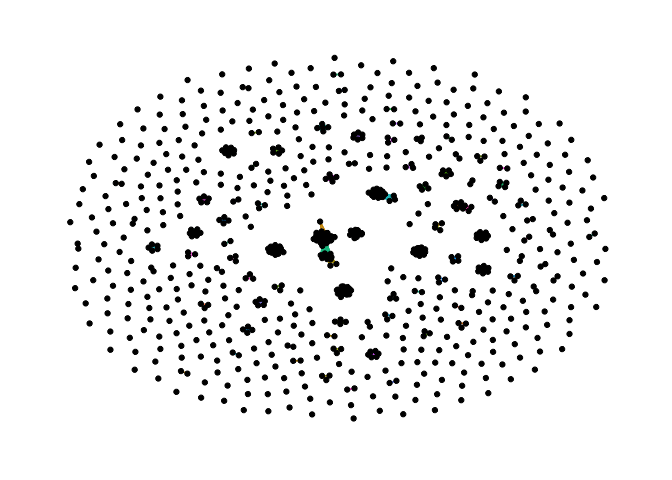
\includegraphics{exercise1_files/figure-latex/unnamed-chunk-4-1.pdf}

\end{document}
